\section{Statisches Verhalten}


\subsection{Statisches Verhalten von Übertragungsgliedern}

Als statisches Verhalten sollen diejenigen Eigenschaften von Regelkreisgliedern und Regelkreisen bezeichnet werden, die nach dem Abklingen von Übergangs- und Einschwingvorgängen gelten.

Das statische Verhalten kann formelmäßig
\begin{equation}\label{eq:2-1}
    Y = f\parentheses*{U, Z_1, Z_2, \ldots}
\end{equation}
oder durch Kennlinien, Kennlinienfelder, Wertetabellen usw. dargestellt werden.

Als Beispiel für die formelmäßige Beschreibung statischen Verhaltens soll der durch einen Schieber mit verstellbarem Querschnitt nach Bild \ref{fig:2-1} fließende Strom \(Q\) einer inkompressiblen Flüssigkeit als Funktion des freien Schieberquerschnitts \(F\) und der Drücke vor und hinter dem Schieber \(P_e\) und \(P_a\) angeschrieben werden.

\begin{figure}[h]
    \centering
    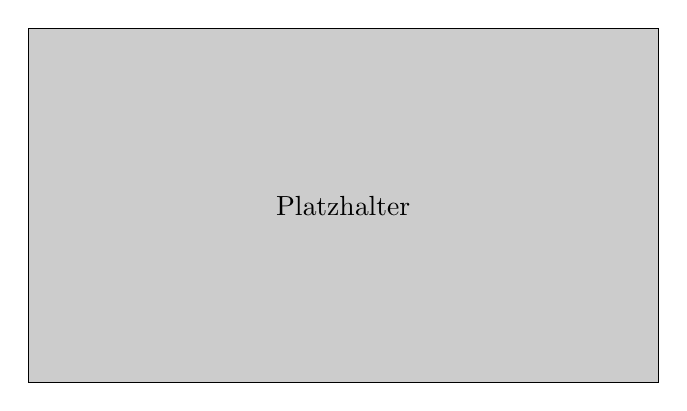
\begin{tikzpicture}
        \filldraw[fill=white!80!black,draw=black] (0,0) rectangle (8,4.5) node[pos=.5] {Platzhalter};
    \end{tikzpicture}
    \caption{Schieber mit veränderlichem Querschnitt}
    \label{fig:2-1}
\end{figure}

Mit dem Satz von Bernoulli erhält man nach Zusammenfassung aller Konstanten zu \(K\) die Beziehung
\begin{equation}
    Q = KF\sqrt{P_e - P_a}.
\end{equation}
Der gleiche Zusammenhang lässt sich graphisch darstellen, z.B. als Kennlinienfeld für den Strom \(Q\) als Funktion der Druckdifferenz \(P = P_e - P_a\) mit der Fläche \(F\) als Parameter (Bild \ref{fig:2-2}).

\begin{figure}[h]
    \centering
    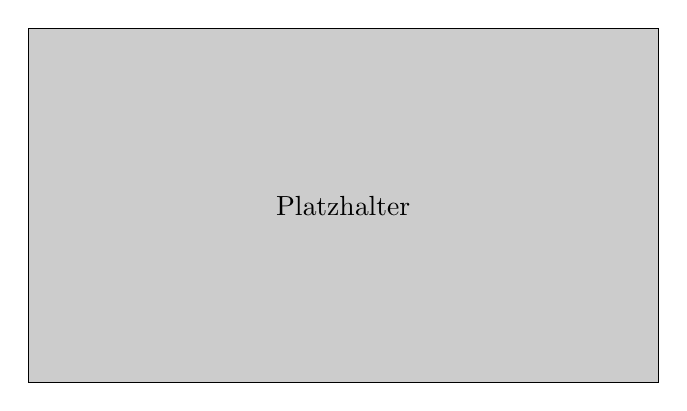
\begin{tikzpicture}
        \filldraw[fill=white!80!black,draw=black] (0,0) rectangle (8,4.5) node[pos=.5] {Platzhalter};
    \end{tikzpicture}
    \caption{Kennlinienfeld eines Schiebers}
    \label{fig:2-2}
\end{figure}


\subsection{Linearisierung, Abweichungsgrößen}

Obgleich die allermeisten technisch wichtigen Zusammenhänge nicht linear sind, strebt man in der Regelungstechnik ihre Linearisierung an.

Lineare Zusammenhänge lassen sich, vor allem bei komplizierten Signalverknüpfungen, wesentlich besser behandeln als nichtlineare.
Daher ist die Linearisierung nichtlinearer Zusammenhänge ein sehr nützliches Werkzeug der Regelungstechnik, obgleich jede Linearisierung nur innerhalb bestimmter Bereiche der beteiligten Größen genügend genau ist.
Weil aber das Ziel einer Regelung häufig darin besteht, Größen innerhalb enger Bereiche zu halten, sorgt in sehr vielen Fällen eine funktionierende Regelung dafür, dass linearisierte Beziehungen zur Beschreibung der interessierenden Zusammenhänge vollauf genügen.
Aus dem gleichen Grund arbeitet die Regelungstechnik vielfach nicht mit den Absolutwerten von Größen, sondern mit Abweichungsgrößen, die im einfachsten Fall als Differenz von Absolutwerten und Bezugswerten gebildet werden.

Als zweckmäßige Bezugswerte haben sich die (konstanten) Werte erwiesen, die Größen dann annehmen, wenn sich das betrachtete System in einem definierten Zustand (Ruhezustand, Normalzustand, Sollzustand) befindet.
Durch solchermaßen festgelegte Werte \(Y_0, U_0, Z_{10}, Z_{20}, \ldots\), die miteinander verträglich sein müssen, wird ein Arbeitspunkt \(A\) definiert.

Im Folgenden wird mit Abweichungsgrößen
\begin{equation}\label{eq:2-3}
    y = Y - Y_0, \quad u = U - U_0, \quad z_1 = Z_1 - Z_{10}, \quad z_2 = Z_2 - Z_{20}, \quad \ldots
\end{equation}
gearbeitet werden, wann immer dies zweckmäßig erscheint.
Zur Unterscheidung von den Absolutwerten werden die Abweichungsgrößen, wie in Gleichung \eqref{eq:2-3}, mit Kleinbuchstaben geschrieben.

In einzelnen Fällen kann es zweckmäßig sein, die Abweichungsgrößen zusätzlich auf konstante Bezugswerte, z.B. Maximalwerte, Arbeitspunktwerte o. Ä. zu normieren.
Normieren auf die Werte im Arbeitspunkt ergibt
\begin{equation}
    \tilde{y} = \frac{Y - Y_0}{Y_0} = \frac{y}{Y_0}, \quad \tilde{u} = \frac{u}{U_0}, \quad \ldots
\end{equation}
Die Möglichkeit der Normierung wird dann genutzt, wenn das Mitführen von Dimensionen keine zusätzliche Klarheit oder Sicherheit vermittelt.
Meist wird jedoch auf ausdrückliche Kennzeichnung normierter Größen verzichtet, weil dies aus dem Zusammenhang hervorgeht.

Durch Linearisieren wird ein vorgegebener nichtlinearer Ausdruck
\[
    Y = f\parentheses*{U, Z_1, Z_2, \ldots}
\]
in der Umgebung eines Arbeitspunktes \(A\) mit
\begin{equation}\label{eq:2-6}
    Y = Y_0, \quad U = U_0, \quad Z_1 = Z_{10}, \quad Z_2 = Z_{20}, \quad \ldots
\end{equation}
durch einen linearen Ausdruck
\begin{equation}
    y = K_u u + K_1 z_1 + K_2 z_2 + \ldots
\end{equation}
mit den Abweichungsgrößen \(y, u, z_1, z_2, \ldots\) und den Konstanten \(K_u, K_1, K_2, \ldots\) ersetzt.

Man erhält die Koeffizienten des linearen Ausdruckes \eqref{eq:2-6} durch eine Taylor-Reihenentwicklung der nichtlinearen Funktion \eqref{eq:2-1}.
Praktisch muss man dazu die (partiellen) Ableitungen der Ausgangsgröße nach den Eingangsgrößen bestimmen. So gewinnt man aus
\begin{equation}\label{eq:2-7}
    y = \brackets*{\frac{\partial Y}{\partial U}}_A u + \brackets*{\frac{\partial Y}{\partial Z_1}}_A z_1 + \brackets*{\frac{\partial Y}{\partial Z_2}}_A z_2 + \ldots
\end{equation}
durch Koeffizientenvergleich
\begin{equation}\label{eq:2-8}
    K_u = \brackets*{\frac{\partial Y}{\partial U}}_A, \quad K_1 = \brackets*{\frac{\partial Y}{\partial Z_1}}_A, \quad K_2 = \brackets*{\frac{\partial Y}{\partial Z_2}}_A, \quad \ldots
\end{equation}
Diese Koeffizienten sind konstante Werte, die nur noch vom Arbeitspunkt abhängen.

Als Beispiel soll die folgende nichtlineare Beziehung linearisiert werden.
\begin{equation}
    Y = \frac{Z^2}{U} + B, \quad B = \text{konst}.
\end{equation}
Mit den Gleichungen \eqref{eq:2-7}, \eqref{eq:2-8} erhält man den linearen Ausdruck
\begin{equation}
    y = -\frac{Z_0^2}{U_0^2}u + \frac{2Z_0}{U_0}z
\end{equation}
mit \(U_0\) und \(Z_0\) als den Arbeitspunktwerten von \(U\) und \(Z\).

Falls der zu linearisierende Zusammenhang in Form einer Kennlinie oder eines Kennlinienfeldes gegeben ist, lassen sich die Koeffizienten des gesuchten linearen Ausdrucks durch näherungsweise Differentiation gewinnen.
Dabei entspricht die Einführung von Abweichungsgrößen der Definition eines neuen Koordinatensystems, dessen Ursprung im Arbeitspunkt (Bild \ref{fig:2-3}).

\begin{figure}[h]
    \centering
    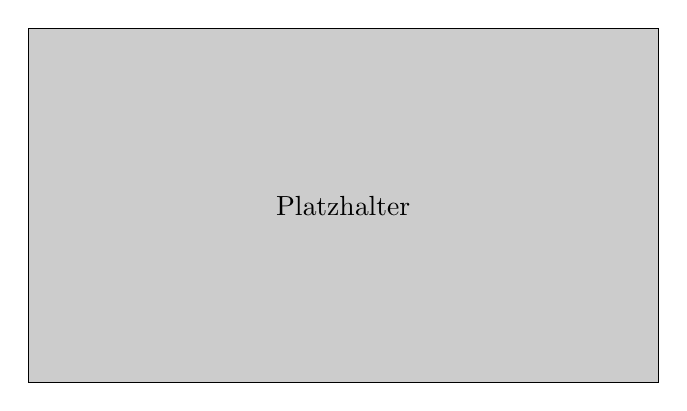
\begin{tikzpicture}
        \filldraw[fill=white!80!black,draw=black] (0,0) rectangle (8,4.5) node[pos=.5] {Platzhalter};
    \end{tikzpicture}
    \caption{Linearisierung einer Kennlinie}
    \label{fig:2-3}
\end{figure}

Die Linearisierung eines durch eine Kennlinie gegebenen Zusammenhanges \(y = f\parentheses*{U}\) zeigt Bild \ref{fig:2-3}.
Die gegebene Kennlinie in dem gegebenen Koordinatensystem wird durch die Gerade \(y = Ku\) in dem neu eingeführten Koordinatensystem der Abweichungsgrößen ersetzt.
Wegen
\begin{equation}
    y = \brackets*{\frac{\partial Y}{\partial U}}_A u = Ku
\end{equation}
ist
\begin{equation}
    K = \brackets*{\frac{\partial Y}{\partial U}}_A,
\end{equation}
d.h. die Steigung der Ersatzgeraden ist gleich der Steigung der Kennlinie im Arbeitspunkt.

Zusammenhänge zwischen einer abhängigen und zwei oder mehreren unabhängigen Größen lassen sich in Kennlinienfeldern darstellen.
Zur näherungsweisen Bestimmung der Ableitung der abhängigen Größe nach einer Größe, die Parameter von Kennlinien ist, benutzt man zweckmäßigerweise einen geeigneten Differenzenquotienten.

\begin{figure}[h]
    \centering
    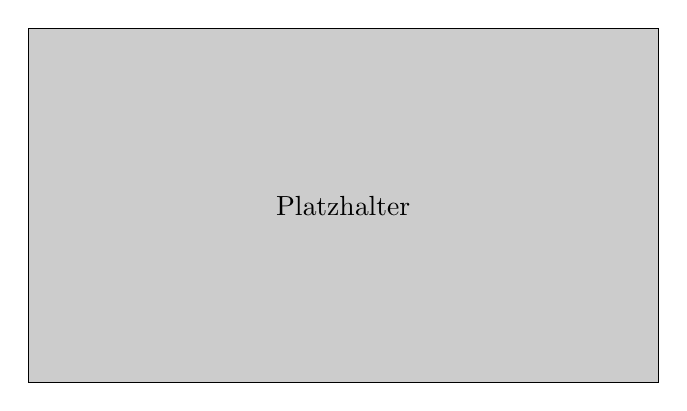
\begin{tikzpicture}
        \filldraw[fill=white!80!black,draw=black] (0,0) rectangle (8,4.5) node[pos=.5] {Platzhalter};
    \end{tikzpicture}
    \caption{Linearisierung eines Kennlinienfeldes}
    \label{fig:2-4}
\end{figure}

Die Linearisierung des in Bild \ref{fig:2-4} dargestellten Kennlinienfeldes liefert die Koeffizienten \(K_u\) und \(K_z\) der linearen Gleichung für Abweichungsgrößen
\begin{equation}
    y = K_u u + K_z z.
\end{equation}
Der Koeffizient \(K_u\) ergibt sich aus der Steigung der Kennlinie für \(Z = Z_0\) im Arbeitspunkt bzw. als Steigung der Tangenten, die die Kennlinie im Arbeitspunkt berührt.
\begin{equation}
    K_u = \brackets*{\frac{\partial Y}{\partial U}}_A = \brackets*{\frac{\Delta Y_u}{\Delta U}}_{Z = Z_0}.
\end{equation}
Um den Koeffizienten \(K_z\) nach dem gleichen Verfahren zu bestimmen zu können, benötigt man eine Kennlinie \(Y = f\parentheses*{Z, U_0}\) mit \(U = U_0\) als Parameter.
Im rechten Teil von Bild \ref{fig:2-4} ist eine solche Kennlinie dargestellt.
Man erkennt, dass der Unterschied zwischen der Steigung und der (nicht eingezeichneten) Tangente im Arbeitspunkt an diese Kennlinie und der Steigung der Sekante durch dei dem Arbeitspunkt benachbarten Punkte \(Y\parentheses*{U_0, Z = 2}\) und \(Y\parentheses*{U_0, Z = 4}\) gering ist.
Bei geeigneter Wahl der Sekante erhält man also nur kleine Fehler, wenn man auf die Tangente verzichtet.
Dieser Schritt liegt nahe, weil die Steigung der Sekante ohne zusätzliche Zeichenarbeit aus dem ursprünglichen Kennlinienfeld (Bild \ref{fig:2-4}, links) bestimmbar ist nach
\begin{equation}
    K_z = \brackets*{\frac{\partial Y}{\partial Z}}_A = \brackets*{\frac{\Delta Y_z}{\Delta Z}}_{U = U_0}.
\end{equation}
Bei dieser Vorgehensweise ist darauf zu achten, das die Sekanten durch Punkte gelegt werden, die in etwa symmetrisch zum Arbeitspunkt liegen und nicht allzu weit von ihm entfernt sind.

Da das Vorzeichen von der Richtung wachsender Werte des Parameters \(Z\) abhängt, ist es wichtig, die Differenzen so zu bilden, dass die zu einem Punkt gehörenden \(Y\)- und \(Z\)-Werte mit gleichem Vorzeichen eingesetzt werden.
Welche Werte dann mit positivem und welche mit negativem Vorzeichen versehen werden, ist gleichgültig, d.h.
\begin{equation}
    K_z \cong \frac{Y\parentheses*{U_0, Z = 4} - Y\parentheses*{U_0, Z = 2}}{\parentheses*{Z = 4} - \parentheses*{Z = 2}} = \frac{Y\parentheses*{U_0, Z = 2} - Y\parentheses*{U_0, Z = 4}}{\parentheses*{Z = 2} - \parentheses*{Z = 4}}.
\end{equation}
Für die Bestimmung der Steigung der Tangente gilt das Gleiche; da deren Vorzeichen leichter zu erkennen ist, ist ein streng formales Vorgehen weniger wichtig.

Oft sind die zu linearisierenden Zusammenhänge nicht in der expliziten Form der Gleichung \eqref{eq:2-1} oder der Bilder \ref{fig:2-3} und \ref{fig:2-4} angegeben.
So können die Zusammenhänge auch durch analytische Ausdrücke oder grafische Darstellungen in impliziter Form wie z.B.
\begin{equation}
    U = f\parentheses*{Y, Z_1, Z_2, \ldots}
\end{equation}
oder
\begin{equation}
    0 = f\parentheses*{Y, U, Z_1, Z_2, \ldots}
\end{equation}
oder
\begin{equation}
    Y = f\parentheses*{Y, U, Z_1, Z_2, \ldots}
\end{equation}
gegeben sein.
Sehr häufig findet man auch Zusammenhänge, die durch mehrere nichtlineare Gleichungen oder Kennlinien(-felder) mit einer der Zahl der Gleichungen entsprechenden Zahl von Zwischenvariablen dargestellt werden.
Diese Zwischenvariablen lassen sich meist nicht einfach eliminieren, z.B. dann nicht wenn eine Gleichung und ein Kennlinienfeld gegeben sind.
Beispiele für Zusammenhänge dieser Art mit einer Zwischenvariablen \(H\) sind
\begin{align}
    \begin{split}
        Y &= g\parentheses*{H, U, \ldots},\\
        H &= f\parentheses*{Y, U, \ldots},\\
        0 &= f\parentheses*{H, Y, U, \ldots}
    \end{split}
\end{align}
kombiniert mit
\begin{align}
    \begin{split}
        H &= g\parentheses*{U, Z, \ldots},\\
        U &= g\parentheses*{H, Z, \ldots},\\
        0 &= g\parentheses*{H, U, Z, \ldots}.
    \end{split}
\end{align}
In allen diesen und ähnlichen Fällen ist zweckmäßigerweise das folgende Verfahren anzuwenden, das aus dem vorher erläuterten unmittelbar folgt:
\begin{enumerate}
    \item Mit den gegebenen nichtlinearen Beziehungen sind alle benötigten Arbeitspunktwerte für alle Variablen zu ermitteln.
    \item Jede gegebene nichtlineare Beziehung (Gleichung oder Kennlinienfeld) ist durch eine vollständige lineare Gleichung zu ersetzen, die durch Linearisierung für den gegebenen Arbeitspunkt entsteht.
    \item Durch Zusammefassen mit Elimination von Zwischenvariablen und Umformen sind die nach 2. gewonnenen linearen Gleichungen in die gewünschte Form, z.B. die der Gleichung \eqref{eq:2-6} zu bringen.
\end{enumerate}
Das Vorgehen soll an einem Beispiel veranschaulicht werden.
Gegeben sei das nichtlineare Gleichungssystem
\begin{align}
    \begin{split}
        H &= f\parentheses*{Y, U},\\
        0 &= g\parentheses*{U, Z, H}.
    \end{split}
\end{align}
Durch Linearisieren erhält man
\begin{align}
    h &= \underbrace{\brackets*{\frac{\partial f\parentheses*{Y, U}}{\partial Y}}_A}_{a_1}y + \underbrace{\brackets*{\frac{\partial f\parentheses*{Y, U}}{\partial U}}_A}_{a_2}u,\\
    0 &= \underbrace{\brackets*{\frac{\partial g\parentheses*{U, Z, H}}{\partial U}}_A}_{b_1}u + \underbrace{\brackets*{\frac{\partial g\parentheses*{U, Z, H}}{\partial Z}}_A}_{b_2}z + \underbrace{\brackets*{\frac{\partial g\parentheses*{U, Z, H}}{\partial H}}_A}_{b_3}h
\end{align}
und durch Einsetzen der oberen Gleichung in die untere
\begin{equation}
    0 = b_1 u + b_2 z + b_3 a_1 y + b_3 a_2 u,
\end{equation}
die nun nach \(y\) aufgelöst
\begin{equation}
    y = -\frac{b_1 + b_3 a_2}{b_3 a_1}u - \frac{b_2}{b_3 a_1}z
\end{equation}
ergibt.

Gelegentlich wird der Übertragungsfaktor einer Regelstrecke (oder eines anderen Regelkreisgliedes) benötigt, die aus mehreren Einzelgliedern mit bekannten Übertragungsfaktoren besteht.
Solche Aufgaben kann man dadurch lösen, dass man die für die Signale zwischen den Einzelgliedern geltenden Beziehungen ansetzt und umformt.
Für die häufig anzutreffenden Parallel-, Reihen- und Rückkopplungsschaltungen gelten die in der später zu verwendenden Tabelle \ref{tab:3_7} für sog. Frequenzgänge zusammengestellten Angaben in analoger Weise.
So ist der Übertragungsfaktor einer Parallelschaltung gleich der Summe und dr einer Reihenschaltung gleich dem Produkt der Übertragungsfaktoren der Einzelglieder.


\subsection{Statisches Verhalten von Regelkreisen}

Aus den statischen Eigenschaften von Regelstrecke und Regler kann man auf das statische Verhalten des Regelkreises schließen.
Es erscheint daher sinnvoll, das statische Verhalten von Regelkreisen zu betrachten, ehe man sich den dynamischen Eigenschaften zuwendet.
Bei der statischen Betrachtungsweise können nichtlineare Abhängigkeiten in gewissem Umfang berücksichtigt werden.
Im Gegensatz dazu beruht eine Untersuchung der dynamischen Eigenschaften in der überwiegenden Mehrzahl aller Fälle auf einer vorangegangenen Linearisierung.

Für die Betrachtung des statischen Verhaltens von Regelkreisen genügt es, zwischen zwei Grundtypen von stetig wirkenden Reglern zu unterscheiden.
Es sind dies zum einen Regler, die i Wesentlichen proportional wirken und die hier durch den so genannten \(P\)-Regler vertreten werden und zum anderen Regler mit integrierend wirkendem Anteil, die hier durch den \(I\)-Regler vertreten werden (Bild \ref{fig:2-5}).
Nicht stetig wirkende Regler sollen später behandelt werden.

\begin{figure}[h]
    \centering
    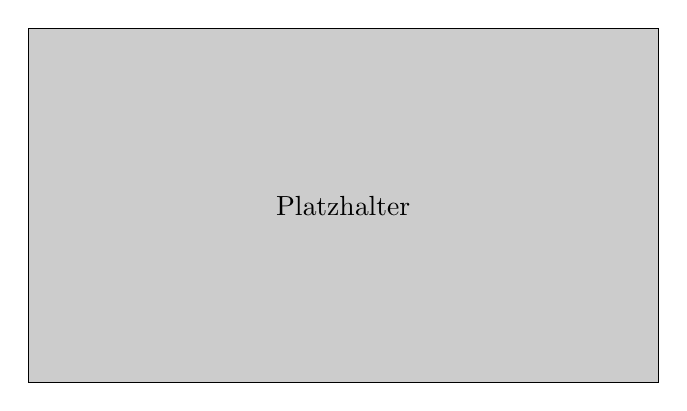
\begin{tikzpicture}
        \filldraw[fill=white!80!black,draw=black] (0,0) rectangle (8,4.5) node[pos=.5] {Platzhalter};
    \end{tikzpicture}
    \caption{Blocksymbole für Regler}
    \label{fig:2-5}
\end{figure}

Der \(P\)-Regler, Proportionalregler oder proportional wirkende Regler arbeitet nach der Gleichung
\begin{equation}
    y = K_R x
\end{equation}
und wird durch das Blocksymbol in Bild \ref{fig:2-5} dargestellt.
Er zeichnet sich dadurch aus, dass er zu jedem Wert der Regelgröße (oder der Regelabweichung) einen durch die angegebene Gleichung bestimmten Wert der Stellgröße \(y\) angibt.

Der \(I\)-Regler, Integralregler oder integrierend wirkende Regler wird durch eine Integralgleichung
\begin{equation}
    y = K_I \int_0^t x\parentheses*{\tau}\d\tau
\end{equation}
oder eine Differentialgleichung
\begin{equation}
    \dot{y} = K_1 x
\end{equation}
und das entsprechende Blocksymbol in Bild \ref{fig:2-5} beschrieben.
Seine wesentlichen Eigenschaften beruhen darauf, dass nicht wie beim \(P\)-Regler die Ausgangsgröße selbst, sondern die Änderungsgeschwindigkeit der Ausgangsgröße proportional der Eingangsgröße ist.
Für eine statische Betrachtung bedeutet dies, dass Übergangs- und Ausgleichsvorgänge erst dann abgeschlossen sind, wenn die Eingangsgröße des \(I\)-Reglers zu Null geworden ist.

Anhand der Kennlinienfelder für zwei Regelstrecken mit unterschiedlichen Eigenschaften soll zum einen die prinzipielle Wirkungsweise beider Eigenschaften soll zum einen die prinzipielle beider Reglertypen verdeutlicht, zum anderen die Auswirkungen  der Wahr des Reglerübertragungsverhaltens auf die technische Brauchbarkeit einer Regelung dargestellt werden.
Da sich das statische Verhalten der Regler ebenfalls durch Kennlinien beschreiben lässt, die in das Kennlinienfeld der Regelstrecke eingetragen werden können (Bilder \ref{fig:2-6} und \ref{fig:2-8}), sind so Aussagen zum statischen Verhalten des geschlossenen Regelkreises möglich.

Bild \ref{fig:2-7} zeigt die Struktur des Regelkreises mit Regler \(R\) und nichtlinearer Regelstrecke \(S\), deren statisches Verhalten durch die Kennlinien im Bild \ref{fig:2-6} beschrieben ist.

\begin{figure}[h]
    \centering
    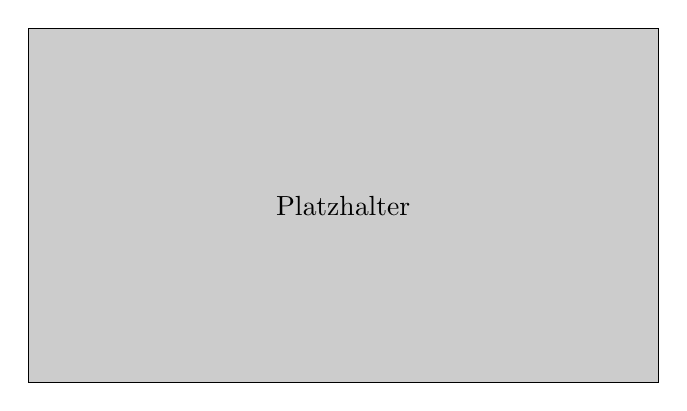
\begin{tikzpicture}
        \filldraw[fill=white!80!black,draw=black] (0,0) rectangle (8,4.5) node[pos=.5] {Platzhalter};
    \end{tikzpicture}
    \caption{Kennlinien von Regelstrecke und Regler}
    \label{fig:2-6}
\end{figure}

\begin{figure}[h]
    \centering
    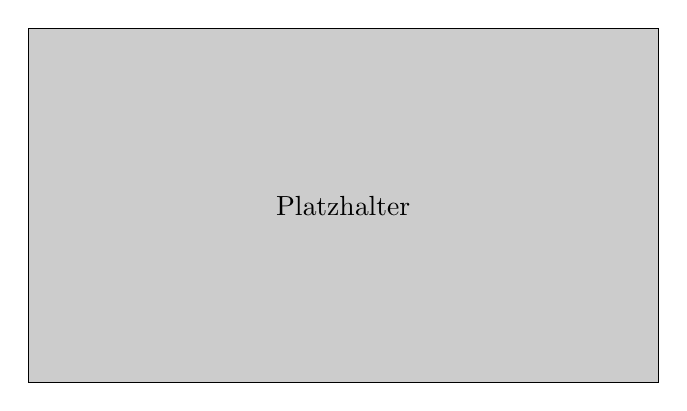
\begin{tikzpicture}
        \filldraw[fill=white!80!black,draw=black] (0,0) rectangle (8,4.5) node[pos=.5] {Platzhalter};
    \end{tikzpicture}
    \caption{Regelkreis mit nichtlinearer Regelstrecke (hier: negatives Stellübertragungsverfahren der Regelstrecke)}
    \label{fig:2-7}
\end{figure}

Für den \(P\)-Regler erhält man aus der Gleichung für Abweichungsgrößen
\begin{equation}
    y = K_R x
\end{equation}
durch Einsetzen
\begin{equation}
    Y - Y_0 = K_R \parentheses*{X - X_0}
\end{equation}
und durch Umstellen
\begin{equation}
    X = X_0 + \frac{1}{K_R}\parentheses*{Y - Y_0}
\end{equation}
die Gleichung einer Geraden mit der Steigung \(\frac{1}{K_R}\), die durch den Punkt \(X_0, Y_0\) geht.

Da der \(I\)-Regler einen Beharrungszustand nur erreicht, wenn die Regelabweichung \(x\) zu Null wird, ergibt sich als ``Kennlinie des \(I\)-Reglers'' die Gerade \(X = X_0\); ein an sich triviales Ergebnis.

Es sollen nun die Änderungen der Regelgröße \(X\) ermittelt werden, die infolge einer Änderung der Störgröße \(Z\) entstehen.
Der Regelkreis möge sich zunächst im Betriebspunkt \(X_0, Y_0\) befinden.
Zu diesem Betriebspunkt gehört kaut Kennlinienfeld eine Störgröße \(Z_0 = 3\).
Die Störgröße möge ihren Wert auf \(Z_1 = 1\) ändern.

Solange die Regelstrecke ohne Regler betrieben wird, ist keine Einrichtung vorhanden, die die Stellgröße \(Y\) verändern könnte; es wird daher \(Y = Y_0\) sein für alle Werte von \(X\) und \(Z\).
Die Regelgröße ist nur von der Störgröße abhängig, und alle Betriebspunkte liegen auf der Vertikalen \(Y = Y_0\).
Der zu \(Z = Z_1 = 1\) gehörende Betriebspunkt ist daher der Schnittpunkt \(1\) dieser Vertikalen mit der Kennlinie der Regelstrecke für \(Z = 1\).

Ein mit der Regelstrecke verbundener \(P\)-Regler wird bei Änderungen der Regelgröße entsprechende Änderungen der Stellgröße verursachen.
Sein statisches Verhalten wird durch seine Kennlinie beschrieben.
Alle Betriebspunkte des Regelkreises müssen daher auf dieser Geraden mit der Steigung \(\frac{1}{K_R}\) liegen.
Der zu \(Z = 1\) gehörende Betriebspunkt ist daher der Schnittpunkt \(2\) der Reglerkennlinie mit der Kennlinie der Regelstrecke für \(Z = 1\).
Ein Vergleich der Regelabweichung ohne Regler \(\Delta X_{oR}\) und der mit \(P\)-Regler \(\Delta X_{mR}\) zeigt, dassdurch den Regler die Auswirkung einer Störgrößenänderung vermindert wird.

Man erkennt weiter, dass die Regelabweichung nicht Null wird, sondern einen endlichen Wert annimmt.
Um die Regelabweichung Null zu erhalten, müsste die Reglerkennlinie waagerecht verlaufen.
Dem würde ein Proportionalbeiwert des Reglers \(K_R \to \infty\) entsprechen, ein Wert, der aus mehreren Gründen nicht erreichbar ist.
Daher kann man feststellen, dass Regelungen mit \(P\)-Reglern eine bleibende Regelabweichung aufweisen.

Da beim Einsatz eines \(I\)-Reglers alle Betriebspunkte auf der Waagerechten \(X = X_0\) liegen müssen, arbeiten Regelungen mit \(I\)-Reglern ohne bleibende Regelabweichung, d.h. Störungen werden durch entsprechend große Änderungen der Stellgröße vollständig ausgeglichen.
Der zu \(Z = 1\) gehörende Betriebspunkt ist daher der Schnittpunkt \(3\) der Linie \(X = X_0\) mit der Kennlinie der Regelstrecke für \(Z = 1\).

Ein Vergleich des statischen Verhaltens geregelter Anlagen mit \(P\)- und \(I\)-Reglern fällt offensichtlich zugunsten des Reglers mit integrierendem Verhalten aus.
Dennoch sind sehr viele Anlagen mit \(P\)-Reglern ausgerüstet, weil neben den statischen auch die dynamischen Eigenschaften und die Gerätekosten eine Rolle bei der Wahl des Reglers spielen.
Pauschal kann man das Verhalten von \(P\)- und \(I\)-Regelungen durch die Aussage charakterisieren, dass \(P\)-Regler auf Störungen bzw. Regelabweichungen rasch reagieren, eine bleibende Regelabweichung aber nicht vermeiden können, während \(I\)-Regler keine bleibende Regelabweichung zulassen, aber nur langsam reagieren.

Zur Charakterisierung der Wirksamkeit einer \(P\)-Regelung bei Störungen dient der Regelfaktor
\begin{equation}
    R = \frac{\Delta X_{mR}}{\Delta X_{oR}}.
\end{equation}
Er ist bei sinnvollen Regelungen kleiner als Eins.
Sein Wert hängt vom Übertragungsfaktor \(K_R\) des Reglers und den Eigenschaften der Regelstrecke ab.
Bei nichtlinearen Regelstrecken, wie der durch das Kennlinienfeld Bild \ref{fig:2-6} beschriebenen, ist der Regelfaktor keine Konstante, sondern von der zugrunde gelegten Störgrößenänderung abhängig.

Im Folgenden soll für eine durch das Kennlinienfeld in Bild \ref{fig:2-8} beschriebene Regelstrecke das statische Verhalten des geschlossenen Regelkreises bei Einsatz eines \(P\)-Reglers mit unterschiedlichem Übertragungsfaktor betrachtet werden.

Beim Vergleich der Kennlinienfelder in Bild \ref{fig:2-8} und Bild \ref{fig:2-6} fällt auf, dass die Kennlinien der Regelstrecke in einem Fall positive und im anderen Fall negative Steigung besitzen.
Man erkennt (ggf. durch Eintragen einer entsprechenden Reglerkennlinie), dass in Bild \ref{fig:2-8} nur Reglerkennlinien mit negativer und in Bild \ref{fig:2-6} nur solche mit positiver Steigung geeignet sind, die bleibende Regelabweichung mit Regler keiner als die ohne Regler werden zu lassen.
D.h. die Steigung der Reglerkennlinie muss ein der Steigung der Regelstreckenkennlinie entgegengesetztes Vorzeichen haben.

\begin{figure}[h]
    \centering
    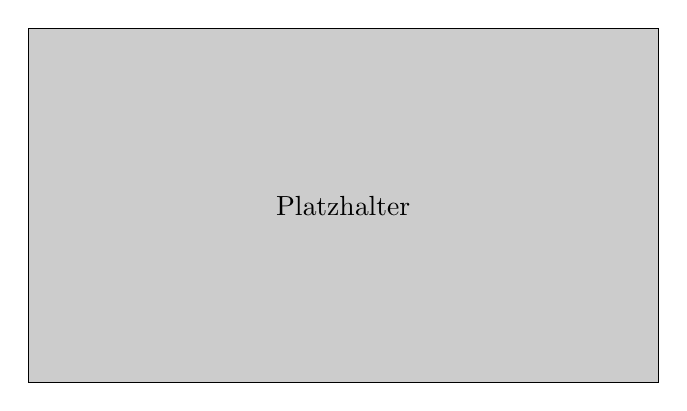
\begin{tikzpicture}
        \filldraw[fill=white!80!black,draw=black] (0,0) rectangle (8,4.5) node[pos=.5] {Platzhalter};
    \end{tikzpicture}
    \caption{Kennlinien von Regelstrecke und \(P\)-Regler mit unterschiedlichem Übertragungsfaktor \(K_R\)}
    \label{fig:2-8}
\end{figure}

\begin{figure}[h]
    \centering
    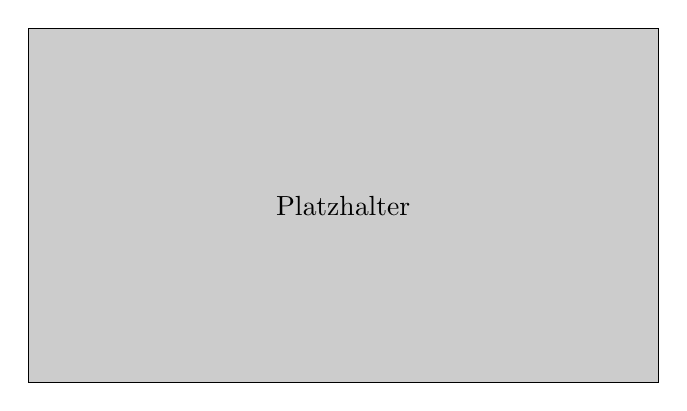
\begin{tikzpicture}
        \filldraw[fill=white!80!black,draw=black] (0,0) rectangle (8,4.5) node[pos=.5] {Platzhalter};
    \end{tikzpicture}
    \caption{Regler mit negativem Übertragungsverhalten}
    \label{fig:2-9}
\end{figure}

Der in Bild \ref{fig:2-7} dargestellte Regler hat positives Übertragungsverhalten, d.h. die Stellgröße \(Y\) wächst mit zunehmender Regelgröße \(X\), wie es auch die Reglerkenngröße in Bild \ref{fig:2-6} zeigt.
Für eine Regelstrecke entsprechend Bild \ref{fig:2-8} ist ein Regler mit negativem Übertragungsverhalten notwendig, der mit zunehmender Regelgröße die Stellgröße verringert; der Regler in Bild \ref{fig:2-9} leistet genau dies.

Im Kennlinienfeld Bild \ref{fig:2-8} sind Reglerkennlinien für unterschiedliche Übertragungsfaktoren \(K_R\) eingetragen.
Man erkennt, dass die bleibende Regelabweichung z.B. für eine Änderung der Störgröße von \(Z_0 = 3\) auf \(Z_1 = 1\) mit steigendem Übertragungsfaktor \(K_R\) abnimmt.
Ferner, dass sie für einen negativen Übertragungsfaktor, dem hier eine Reglerkennlinie mit positver Steigung entspricht, sogar größer wird, als im Fall ohne Regler.
Für den Regelfaktor gilt das Entsprechende.

Für technisch sinnvolle Regelungen wird fast immer ein Regelfaktor gefordert, der keiner ist als etwa \(0,2\), d.h. eine Regelung sollte die Wirkung von Störgrößen auf etwa \(20\%\) des Wertes ohne Regelung vermindern können, um den notwendigen Aufwand zu rechtfertigen.

Für Regelkreise mit linearen Regelstrecken oder für linearisierte Zusammenhänge zwischen Regel-, Stell- und Störgrößen lässt sich der Regelfaktor formelmäßig bestimmen.

\begin{figure}[h]
    \centering
    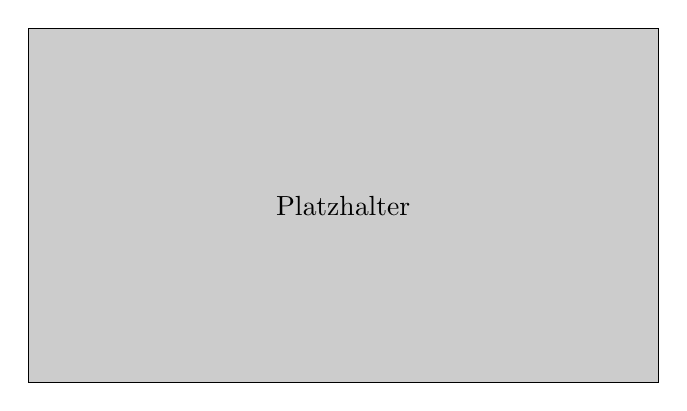
\begin{tikzpicture}
        \filldraw[fill=white!80!black,draw=black] (0,0) rectangle (8,4.5) node[pos=.5] {Platzhalter};
    \end{tikzpicture}
    \caption{Linearer Regelkreis}
    \label{fig:2-10}
\end{figure}

Bild \ref{fig:2-10} zeigt den Wirkungsplan eines linearen Regelkreises.
Das statische Verhalten der Regelstrecke wirddurch die Gleichung
\begin{equation}
    x = -K_y y + K_z z,
\end{equation}
das des Reglers durch
\begin{equation}
    y = K_R x
\end{equation}
beschrieben.
Die Führungsgröße \(w\) ist zu Null gesetzt und daher fortgelassen worden, weil sie ohne Einfluss auf das Folgende ist.

Für die Regelstrecke ohne Regler gilt der statische Zusammenhang
\begin{equation}\label{eq:2-36}
    x_{oR} = K_z z,
\end{equation}
weil wegen des fehlenden Reglers \(y = 0\) ist.

Für den Regelkreis aus Regler und Strecke gelten die Gleichungen für beide Glieder.
\begin{align}
    x_{mR} &= -K_y y_{mR} + K_z z,\\
    y_{mR} &= K_R x_{mR}.
\end{align}
Da \(x_{mR} = f\parentheses*{z}\) interessiert, ist \(y_{mR}\) zu eliminieren.
Einsetzen ergibt
\begin{equation}
    x_{mR} = -K_y K_R x_{mR} + K_z z,
\end{equation}
und nach Umformung erhält man
\begin{equation}\label{eq:2-40}
    x_{mR} = \frac{K_z}{1 + K_y K_R}z.
\end{equation}
In Gleichung \eqref{eq:2-40} ist das Produkt \(K_y K_R\) der Übertragungsfaktor der Reihenschaltung von Regelstrecke zu Regler.
Aus Gleichung \eqref{eq:2-36} und \eqref{eq:2-40} ergibt sich der Regelfaktor für lineare bzw. linearisierte Regelkreise zu
\begin{equation}\label{eq:2-41}
    R = \frac{\Delta X_{mR}}{\Delta X_{oR}} = \frac{x_{mR}}{x_{oR}} = \frac{K_z}{1 + K_y K_R}z\frac{1}{K_z z} = \frac{1}{1 + K_y K_R},
\end{equation}
d.h. er hängt nur noch von den Übertragungsfaktoren \(K_y\) und \(K_R\) ab.
Ach hier gilt, dass der Regelfaktor mit wachsendem Übertragungsfaktor \(K_R\) des Reglers bzw. mit wachsendem Produkt \(K_y K_R\) der Übertragungsfaktoren von Regler und Regelstrecke abnimmt.

Als Beispiel soll das statische Verhalten eines Generators mit Spannungsregelung nach Bild \ref{fig:2-11} behandelt werden.
Der Generator wird mit konstanter Frehzahl angetrieben.
Die von ihm abgegebene Spannung \(U\) hängt entsprechend dem Kennlinienfeld von der Stromaufnahme \(I_A\) (Ankerstrom) der angeschlossenen Verbraucher und dem Erregerstrom \(I_e\) ab.
Die Regeleinrichtung besteht aus einer Konstantspannungsquelle (Batterie), die die Sollspannung \(U_0\) liefert, und einem elektronischen Verstärker, der aus der Spannungsabweichung \(U_R\) entsprechend der gegebenen Kennlinie den Erregerstrom \(I_e\) erzeugt.

\begin{figure}[h]
    \centering
    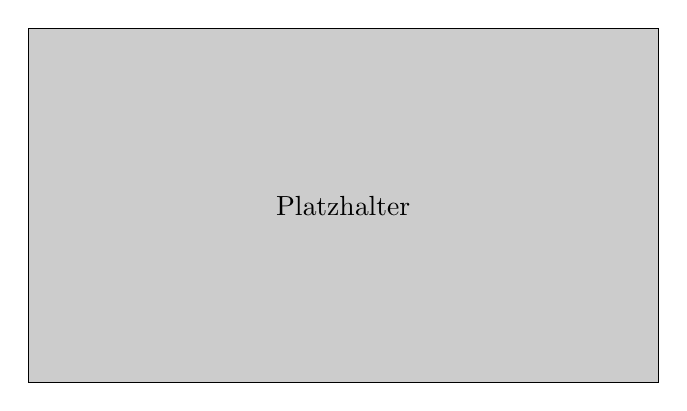
\begin{tikzpicture}
        \filldraw[fill=white!80!black,draw=black] (0,0) rectangle (8,4.5) node[pos=.5] {Platzhalter};
    \end{tikzpicture}
    \caption{Generator mit Spannungsregelung, Anlagenschema und Kennlinien}
    \label{fig:2-11}
\end{figure}

Der Generator soll zunächst ohne Regelung betrieben werden.
Dazu wird der eingezeichnete Schalter geöffnet, der Regelkreis aufgetrennt und die Spannung am Regler damit \(U_R = 0\sis{\volt}\).
Der Regler liefert entsprechend seiner Kennlinie einen Strom von \(I_e= 0,6\sis{\ampere}\) ohne Rücksicht auf die vom Generator erzeugte Spannung.
Diese Spannung beträgt lt. Kennlinienfeld in Leerlauf \(U_1 = 115\sis{\volt}\); sie sinkt mit zunehmender Last und beträgt bei Volllast \(U_2 = 76\sis{\volt}\).

Die soeben ermittelte Änderung der Spannung bei Belastung ist für viele Zwecke zu groß; durch Schließen des Schalters wird daher die Regelung eingeschaltet.
Als Führungsgröße wird an der Batterie \(U_0 = 100\sis{\volt}\) eingestellt.
Für \(U = U_0\) wird \(U_R = 0\sis{\volt}\) und damit \(I_e = I_{e0} = 0,6\sis{\ampere}\).
Damit liegt der Arbeitspunkt der Regelung fest; aus dem Kennlinienfeld erhält man noch \(I_{A0} = 30\sis{\ampere}\) als Belastung im Arbeitspunkt.
Um die Regelung besser untersuchen zu können, wird die Reglerkennlinie in das Kennlinienfeld übertragen.
Dazu kann man die Kenntnis benutzen, dass diese Kennlinie eine Gerade ist, die durch den Arbeitspunkt verläuft und dass \(I_e\parentheses*{U_R = 10\sis{\volt}} = 0\sis{\ampere}\) ist.
Dem Kennlinienfeld ist zu entnehmen, dass nun bei Leerlauf \(U_3 = 104\sis{\volt}\) und bei Volllast \(U_4 = 93\sis{\volt}\) wird.
Als Regelfaktor erhält man
\begin{equation}\label{eq:2-42}
    R = \frac{U_3 - U_4}{U_1 - U_2} = \frac{104\sis{\volt} - 93\sis{\volt}}{115\sis{\volt} - 76\sis{\volt}} = 0,28,
\end{equation}
d.h. die Auswirkung einer Änderung der Belastung von Leerlauf auf Volllast wird durch die Regelung auf \(28\%\) ihres Wertes ohne Regelung vermindert; für viele technische Zwecke ist ein solcher Regelfaktor allerdings noch zu groß.

Durch Linearisieren der im Kennlinienfeld gegebenen Zusammenhänge kann man für die Beziehung
\begin{equation}
    u = K_y i_e + K_z i_A
\end{equation}
den Wert des Koeffizienten \(K_y\) zu
\begin{equation}
    K_y = \frac{U_0 - U_5}{I_{e0} - I_{e5}} = \frac{100\sis{\volt} - 77\sis{\volt}}{0,6\sis{\ampere} - 0\sis{\ampere}} = 38,3\sis{\volt\per\ampere}
\end{equation}
und aus der Kennlinie des Reglers für
\begin{equation}
    i_e = -K_R u
\end{equation}
den Übertragungsfaktor
\begin{equation}
    K_R = -\frac{\Delta I_e}{\Delta U} = -\frac{-0,6\sis{\ampere}}{10\sis{\volt}} = 0,06\sis{\ampere\per\volt}
\end{equation}
erhalten.
Mit diesen Werten und der Gleichung \eqref{eq:2-41} ergibt sich der Regelfaktor zu
\begin{equation}
    R = \frac{1}{1 + K_y K_R} = \frac{1}{1 + 38,3\sis{\volt\per\ampere} \cdot 0,06\sis{\ampere\per\volt}} = 0,3.
\end{equation}
Dieser Wert stimmt mit dem vorher in Gleichung \eqref{eq:2-42} bestimmten in etwa überein.


\subsection{Stellbereich und Regelbereich}

Im vorangegangenen Abschnitt wurde das statische Verhalten beim Zusammenwirken linearer Regler mit nichtlinearen Regelstrecken bzw. deren linearer Ersatzmodelle betrachtet.
Die Linearität, die dem Regler dabei stets zugeschrieben wird, entspricht dem mathematisch definierten Übertragungsverhalten.
Im einfachsten Fall des linearen \(P\)-Reglers ist die Kennlinie einer Gerade mit positiver oder negativer Steigung.

Bei der technischen Umsetzung ist jedoch zu berücksichtigen, dass die Stell- und Regelgrößen gerätetechnisch bedingten Beschränkungen unterliegen, die durch
\begin{itemize}
    \item den Stellbereich \(Y_h\) (Arbeitsbereich des Stellgeräts, der Ausgangsseite des Reglers)
    \item den Regelbereich \(X_h\) (Arbeitsbereich des Messgeräts, der Eingangsseite des Reglers)
\end{itemize}
vorgegeben werden.
Wie in Bild \ref{fig:2-12} skizziert, wird durch die Beschränkungen des Stell- und Regelbereichs im Kennlinienfeld ein Rechteckfenster beschrieben, in dessen Innern die Kennlinie eines \(P\)-Reglers der bekannten schräg liegenden Gerade folgt, während die Kennlinie beim Verlassen des Fensters in einen horizontalen Verlauf übergeht.
Natürlich sollten Mess- und Stellgeräte so dimensioniert sein, dass deren Beschränkungen im normalen Betrieb eines geregelten Prozesses möglichst nicht erreicht werden.

Als quantitatives Maß, welches neben dem Übertragungsfaktor \(K_R\) zur Kennzeichnung des statischen Übertragungsverhalten von \(P\)-Reglern genutzt wird und den Einfluss etwaiger Beschränkungen durch den Stell- oder Regelbereich einbezieht, dient der Proportionalbereich \(X_P\).
Er wird entweder in Einheiten der Regelgröße oder häufiger als bezogener Proportionalbereich in Prozent angegeben.

\begin{figure}[h]
    \centering
    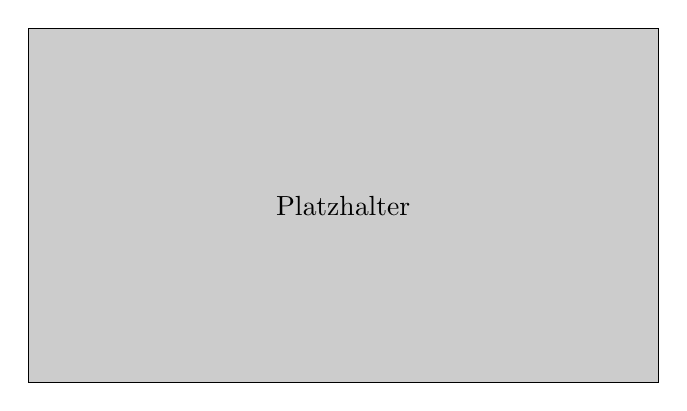
\begin{tikzpicture}
        \filldraw[fill=white!80!black,draw=black] (0,0) rectangle (8,4.5) node[pos=.5] {Platzhalter};
    \end{tikzpicture}
    \caption{Kennlinie eines \(P\)-Reglers mit Stell- und Regelbereich}
    \label{fig:2-12}
\end{figure}

Bild \ref{fig:2-12} zeigt die Kennlinie einer Regeleinrichtung, die außer dem Regler u. U. noch einen Messumformer, ein Stellglied und andere Zusatzgeräte umfassen kann.
Die Geräte sind so ausgelegt, dass die Eingangsgröße \(X_1 \le X \le X_2\) und die Ausgangsgröße \(Y_1 \le Y \le Y_2\) sein muss.
Eingangsgrößen außerhalb des so festgelegten Regelbereiches von der Größe \(X_h\) werden nicht erfasst, und die Stellgröße ist auf den Stellbereich von der Größe \(Y_h\) beschränkt.
Der Bereich \(a\), den die Regelgröße durchlaufen muss, damit als Folge davon die Stellgröße von \(Y_1\) nach \(Y_2\) geändert wird, d.h. den gesamten Stellbereich des Reglers bzw. der Regeleinrichtung durchläuft, wird gelegentlich als Proportionalbereich des Reglers bzw. der Regeleinrichtung bezeichnet.
Dieser Bereich kann je nach Größe des Übertragungsfaktors \(K_R\) größer oder kleiner sein als der Regelbereich \(X_h\).

Als Proportionalbereich soll im Folgenden der bezogene Wert
\begin{equation}
    X_P = \frac{a}{X_h} \cdot 100\%
\end{equation}
bezeichnet werden.
Weil
\begin{equation}
    K_R = \frac{Y_h}{a},
\end{equation}
erhält man
\begin{equation}
    X_P = \frac{Y_h}{X_h K_R} \cdot 100\%.
\end{equation}
Werte von \(1\% \le X_P \le 500\%\) können zu technisch sinnvollen Regelungen gehören.
Da \(X_P\) umgekehrt proportional zu \(K_R\) ist
\begin{equation}
    X_P = \frac{1}{K_R} \cdot \text{konst.},
\end{equation}
ist es wichtig, beim Arbeiten mit Geräten, die nur Skalen für \(X_P\) haben, zu beachten, dass eine Vergrößerung von \(X_P\) einer Verkleinerung von \(K_R\) entspricht und umgekehrt.
